%% 
%% If you intend to use figures of formats jpg, png or pdf and want the 
%% output to be immediately a pdf file, compile with pdflatex. 
%% 
%% If you want to use eps or ps figures, your output will be a dvi 
%% file that can be converted to ps and pdf formats. In this case you 
%% should compile your document with latex. 
%% 
%%This template is compatible with both methods. 
%% 
 
 
\documentclass[a4paper]{IEEEtran} 
\usepackage{pdfpages} 
\usepackage[utf8]{inputenc} 
\usepackage[T1]{fontenc} 
\usepackage{graphicx} 
\usepackage{amsmath} 
\usepackage{amsfonts} 
\usepackage{caption} 
\usepackage{url} 
\usepackage{subcaption} 
\usepackage[caption=false, ...]{subfig} 
 
 
 
 
\title{{ \normalsize Master Thesis} \\ 
GEFILOC: Generic Framework for Indoor Location Systems} 
\author{ 
Ricardo Martins {\tt ricardo.pachecomartins@gmail.com} 
Instituto Superior T\'{e}cnico} 
\date{\today} 
 
 
\begin{document} 
\maketitle 
 
 
\begin{abstract} 
 
 
Nowadays there is a great demand for positioning systems and while the outdoor performance is amazing through the use of GPS, indoor positioning systems have been studied in order to also achieve such results. In this paper one studies the actual state of indoor systems, through an analysis on the usable technologies and techniques. A critical analysis is conducted through a modern perspective centered on location services through smartphones. Since there is a great number of different indoor location systems, one found a need to create a framework capable of hosting such systems in the form of a smartphone-centric architecture. This generic architecture attempted to achieve  interoperability  through the isolation of the main components of indoor systems. As such GEFILOC, a generic framework for indoor location systems, was created. GEFILOC would allow for systems that made use of it, to be capable of operating together on the same device without additional requirements. In order to test the proposed framework, a Bluetooth low energy-based system was implemented. This implementation allowed for analysing the energetic costs of the architecture and comprehending how to set up one or more systems for analysing the interoperability component.  
 
 
\end{abstract} 
 
 
\section{Introduction} 
\label{sec:Introduction} 
 
 
Outdoor positioning systems have greatly evolved in the past with the global positioning system (GPS) as its most important system. Since GPS is an outdoor position systems based on a network of satellite, when it's used for indoor location, it isn't capable of having the same performance. This is caused by the constraints introduced by indoor environments such as attenuation and reflection of electromagnetic waves upon collision with building walls and obstacles \cite{survey1}. As such there was a need to find reliable indoor systems that by nature would reduce the impact of some of the mentioned constraints. 
 
 
In order to understand indoor position there is a need to understand the full scope of variables that comes to surface when moving from outdoor to indoor. When developing an indoor system there is a need to make sure that it can tackle the challenges such as small space dimension which reinforce the need for higher precision, a higher probability of non existent line of sight, influence of obstacles such as walls, furniture, moveable objects such as doors and human beings\cite{reviewtechniques, survey3}. All of the previously mentioned affect the way electromagnetic waves propagate in an indoor environment leading to problems related to severe multipath and reflection on existent surfaces \cite{surveywireless}. Besides propagation challenges, there are energy consumption, accuracy and deployment costs that play a critical role in deciding the viability of a proposed indoor location technique. Another interesting challenges that also surfaces is the means to describe a location. When dealing with outdoor location systems, the provided location is always characterised by two values, latitude and longitude, since the existent environment, i.e. the planet Earth, is always the same and as such the coordinates system can be relative to it. In indoor systems, there are many different types of surrounding environments and as such different ways of representing the data are necessary. If one thinks about providing indoor location on an office, the precise location isn't as relevant as just knowing the general location, i.e. a building specific description of the location in the form of building, floor and room. On other environments such as supermarkets or even in the previous example, where the objective is to provide more a precise location description, a cartesian coordinate system (x,y) is required. 
 
 
With the evolution of mobile devices there has been a sizeable number of different technologies that can possibly be used in indoor location \cite{surveythesis,survey2} such as GPS-based technologies, using high sensitivity antenas to overcome GPS's indoor issues, RFID , Wireless LAN and Bluetooth among others, allowing even for hybrid systems which make use of more than one of the technologies mentioned above.  
 
 
We are now in an era dominated by smartphones and as such they have became the central piece of several indoor location system. Smartphone's evolution allowed for developing system which rely on its sensors and processing capacities to present a solution that isn't dependent on specific hardware. With such a dependency, the first condition that is imposed onto the systems is the compatibility with smartphones, i.e. the required sensors needs to exist on the generic hardware of smartphones. Once this barrier is surpassed, these generic system's are immediately faced with three fundamental questions which will define the architecture of the system and which can be seen on figure \ref{fig:choices}. The first question, Technology, defines the technology that is to be used in conjunction with the smartphone and consequently the way that location data is to be collected. There is a wide range of possibilities for this choice, be it BLE beacons, Wi-Fi Access points, LED lamps or just the microphone for sound collection, and each has an impact on the way that the system functions and on its performance. The second question is the location algorithm, which fundamentally depends on the target requirements of the system, if it's required to provide accurate location of a user or if a more descriptive location, such as the room in which the user is located, is enough. The third and last question is about which way will the location be described, with the existent possibilities having previously been presented.  
 
 
\begin{figure}[htp] 
\centering 
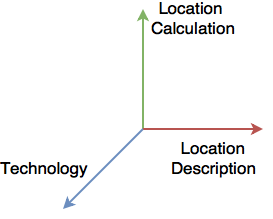
\includegraphics[width=0.5\linewidth]{figures/vectors.png} 
\caption[]{Three fundamental choices in Indoor systems} 
\label{fig:choices} 
\end{figure} 
 
 
When taking into consideration every possible technology and existent algorithm that are capable of being applied on indoor location, we find ourselves with a wide variety of solutions. This high number of variations has led to an increase in the number of existing surveys which attempt to gather make a collection of what has been achieved in the field. Looking at this opportunity one saw the possibility of attempting to create a generic platform capable of being used by any existing indoor location system. In order to implement and test the solution there was a need to decide on which technology to be used and as such one opted by the bluetooth low energy. 
 
 
The idealised generic architecture, which can be seen on figure \ref{fig:generic}, was created with the intention of providing a common ground for any systems which planned to have an indoor location based on a smartphone. It would allow for interoperability among those who make use of it, while presenting a way to structure the system so that the impact on the smartphone is reduced. If one analyses it according to the three points presented in figure \ref{fig:choices}, one can say that by having dedicated servers for the location calculation and the location description instead of having it locally on the smartphone, interoperability is highly improved. This setup allows for systems to implement whichever algorithm they intent, for as long as the server is capable of distinguishing which algorithm is to be used. In scenarios of interoperability, the smartphone should be able to use any of its sensors to capture data, dealing with the technology component, and tag them before sending it for computation on the server. The location description is contained on the map server and it is up to the system to choose which one to use, be it self-created or owned by a third party such as google maps or openstreet maps. For as long as the smartphone is aware of the type of location that he is to receive, interoperability should be achieved. 
 
\begin{figure} 
\centering 
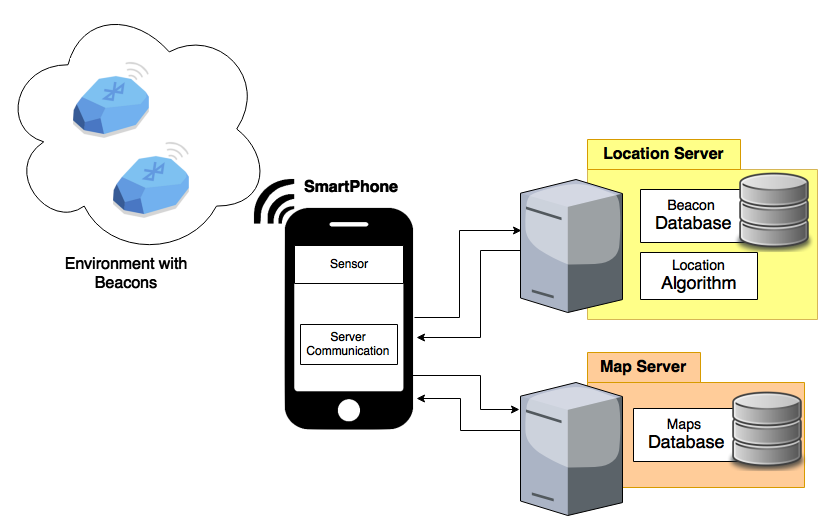
\includegraphics[width=1\linewidth]{figures/generic.png} 
\caption[Generic System's Architecture]{Generic System's Architecture} 
\label{fig:generic} 
\end{figure} 
 
This paper is structured in a way that in section \ref{sec:related} an overview of existent indoor location systems, generic and dedicated, is given, followed by an analyses on the existent location techniques and the ways to describe a location. Section \ref{sec:system} is entirely dedicated to the GEFILOC. The section starts by describing the framework's requirements in subsection \ref{subsec:deployment}, followed by an overview of the architecture in subsection \ref{subsec:architecture}. Subsection \ref{sec:struture} presents the Bluetooth low energy implemented system, while subsection \ref{sec:eval} presents a critical analysis on the implemented system's energetic consumption.  
 
 
\section{Related Word} 
\label{sec:related} 
 
 
In this chapter one will first analyse the systems that laid the foundations of indoor location systems in section \ref{subsec:dedicated}, in order to study systems that were fully dependent on having specific hardware for obtaining user location. Section \ref{subsec:gentech} will present the technologies that are compatible with modern day smartphones, analyse its pros and cons and mention existent projects based on them. The following section, \ref{subsec:tecnique} will describe the existent ways of obtaining the data that is required for inferring a user's location as well as the techniques that make use of them. To conclude, on section \ref{subsec:description}, one will present the existent ways of describing locations through system that make use of them. 
 
 
\subsection{Dedicated Technologies} 
\label{subsec:dedicated} 
 
 
In 1992 the Active badge system \cite{badge} was presented as an infrared solution which was capable of provided room-based position tracking, due to infrared signals being unable to travel through walls. This system imposed users to carry with them an ID card equipped with an IR LED which emitted a signal each fifteen seconds \cite{badge1, badge2}. The long signal frequency was due to the chance of collision of signals from multiple users in the same location while also keeping in mind energy cost, which need to be kept as low as possible. One of the downsides was the decrease in accuracy as the user's location is only known at best to a 15-second window. The user's location was obtained  through the implementation of a network of sensors, which acted as receivers and forwarded the obtained information to the master station. The master station was responsible for polling the sensors, processing data and then making it available to users. One of the biggest issues that were raised with this system was the privacy concerns raised by the clients due to its object tracking nature. 
 
 
At the beginning of the twentieth century, two remarkable projects were presented, Bat system \cite{bat} and RADAR\cite{radar}. The first one, Bat Ultrasonic Location System, was a system capable of tracking various objects, each with a small wireless device called bat \cite{bat1, bat2}. A bat consisted of a radio transmitter with a unique identifier and was meant to be carried by personnel or attached to objects. For locating a bat, the base station periodically transmitted a signal with a single ID which caused the corresponding bat to emit an ultrasound pulse. This pulse was then captured by an existing grid of receivers, which were placed on the ceiling of the areas to be covered, which recorded the time of arrival of the ultrasound. Since the speed of sound in the air is known, the system was capable of converting the time of flight of the ultrasound into distances, in order to obtain the bat's location. 
 
 
The Radar system is a RF-based system to locate and track users inside buildings. The system is divided into two phases, an offline phase used for data collection and a real-time phase where a location is obtained \cite{radar1}. For data collection the mobile application and the base stations are synchronised, in order to be able to obtain time stamps and then the mobile user periodically emits UDP packets to the base stations (BS) . Each BS recorded the RF signal strength measurement together with the time stamp, in order to create a fingerprint of the map.  The real-time phase utilises the real-time user's packet associated RF signal strength, that is obtained at each base station. This information is then forwarded to the central computer where the computation is made. 
 
The last remarkable project, Cricket, managed to tackled some of the problems presented in the last mentioned systems \cite{cricket1}. Each node in the cricket system is composed of a RF transceiver and hardware capable of generating and receiving ultrasonic signals. There are two types of nodes, beacons, which are fixed reference points and are attached to the ceiling or walls of the building, and listeners which are attached to the objects that need to be tracked. Each beacon periodically transmits a RF signal message containing beacon specific information, such as unique ID and beacon position. Whenever a RF signal is transmitted, an ultrasonic pulse is also emitted which enables listeners to measure their distance to the beacons by using the time difference of arrival times of the RF and ultrasonic signals. Each listener utilizes the RF signal's beacon information alongside the obtain distances to beacons to compute their space position and orientation. Cricket's architecture allowed to solve the user privacy, decentralised and ease of deployment issues there were present in the remaining projects \cite{cricket}. 
 
 
\subsection{Generic Technologies} 
\label{subsec:gentech} 
 
 
Wi-Fi is a technology that can be used to estimate the location of a mobile user that resides inside the network. Nowadays Wi-Fi positioning systems have became the most widespread approach for indoor location systems since its access points are readily available in many indoor environments and since all smartphones are equipped with a Wi-Fi antenna they can be located without the need of installing extra software or manipulating the hardware. One issue of Wi-Fi signals is that they suffer attenuation from static environment such as walls and movement of furniture and doors. The most widely location technique used is the radio signal strength indicator (RSSI), which suffers from severe multi-path effects leading to propagation model failures and as such inaccuracy in distance measurement. With these problems in mind a technique called RSSI-based fingerprinting is often used in order to improve performance, the same technique used in the Radar system. 
 
 
Infrared (IR) systems are mostly used for tracking objects or people. IR wavelengths are invisible to the human eye under most circumstances, making this technology less intrusive than those which are visible. This technology is completely available in all smartphones since it makes use of the camera for data input, requiring only line-of-sight communication between receiver and transmitter, preferably without interference from strong light sources. One example of an IR system is Epsilon \cite{epsilon}, which makes use of Light-emitting Diode (LED) and light sensors. Epsilon presents a solution which is easy to use in today's world due to the availability of LED lighting in indoor environments, with the only requirement being the adaptation of the existing infrastructure to the required by the system. In order for the system to work, it required the mobile user to carry a device with an incorporated light sensor, which is the case of pretty much any existent smartphone. 
 
 
Bluetooth is a wireless technology that was created in 1994 with the objective of replacing cables connecting fixed or portable devices. The Bluetooth Low Energy protocol was introduced with the Bluetooth Core Specification version 4 (also called Bluetooth Smart) \cite{BLECore} and it stood out for its lower power consumption, lower complexity and lower cost, while allowing for  device discovery, connection establishment and connection mechanisms.  
 
 
 
 
 
 
 \begin{figure}[htp] 
\centering 
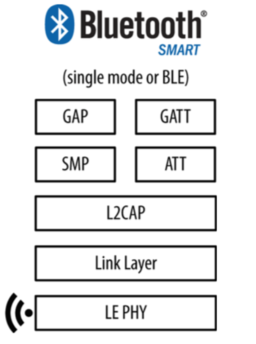
\includegraphics[width=0.5\linewidth]{figures/BLEArchitecture.png} 
\caption[Bluetooth Low Energy Architecture]{Bluetooth low energy architecture} 
\label{fig:BLEarchitecture} 
\end{figure} 
 
 
 
 
When looking at what's possible to achieve using the BLE technology there is the example of Apple's creation iBeacon \cite{ibeacon} which was presented in 2013 with the purpose of implementing proximity sensing systems. The device is capable of being a broadcaster, whose objective is to send information to nearby compatible receivers. The iBeacon can be used to track customers or trigger location-based actions on devices such as push notifications or checking in on social media. As an example, McDonalds used iBeacons to offer special offers to their customers in their fast-food stores. An indoor location system using this technology was presented by Jingjing Yang et al \cite{ibeacon1}, where these devices were used to indicate a patient of his whereabouts through the proximity sensing properties. The user's location was later transferred to a server in order to give clients a variety of different services, from patient counting, to nearby department's information and offer indoor guidance to the nearest available bed.  
 
 
When employing BLE for indoor location, the usual metric used to calculate distances is the RSSI. This metric within the context of Bluetooth brings to surface several issues such as the fact that RSSI as a metric is very accurate only when the target is within a meter of the beacon, since the value decreases as the inverse of the square of the distance to the beacon. As such when developing solutions for indoor location that require systems with high accuracy, capable of tracking moving objects, the usage of RSSI isn't viable without further work. Faragher et al \cite{bleacc} tackled one of the techniques used to improve BLE system's accuracy, fingerprinting, by verifying the effects caused by the device deployment density within the required location. This experiment also puts into evidence one of the downsides of the Bluetooth technology being that its scalability is low. Due to their low range, in order to increase accuracy, an higher density is required . 
 
Zonith \cite{zonith} introduced a Bluetooth based location system with the objective of tracking the position of workers in dangerous environments. Any device registered in the zonith implemented network would be continuously tracked and accounted for in each of the system's functionalities. The system's functionalities involve sounding an alarm whenever a lone worker doesn't move or respond within a time interval (Lone worker protection) or providing a quick a precise location of any worker that has requested for help. This system's deployment requires a study on the best locations for placing the beacons and on the number of required beacons, so that it can provide enough coverage and assure the system's quality. 
 
 
\subsection{Location Calculation techniques} 
\label{subsec:tecnique} 
 
 
The location of a user can be obtained through several different techniques, with each possibility leading to different levels of accuracy and hardware and computational costs. 
The first technique would be proximity detection which has Cell of Origin (CoO) as its most famous technique and allows for room-based detection by assuming that the mobile target is at the cell with the strongest receiving power. This technique is widely used by system using RFID, Bluetooth and Infrared and has low deployment costs as the number of beacons required is small, at least one per room.  
The following technique would be triangulation which uses the geometric properties of the triangle to obtain a position. The metrics used in the position's calculation can be angle-based, which have high implementation costs due to the required antenna's complexity; time-based, using Time-of-flight (ToF) or Round Trip Time (RTT) to obtain measures of distance from beacons; signal property based, using received signal strength indicator (RSSI), although it's only possible of using this metric with radio signals; dead reckoning, which calculates the actual position through the last determined position and an estimate of the device's speed. 
 
 
\subsection{Location Description} 
\label{subsec:description} 
 
 
In order to better understand the existent ways of describing locations it's better to look at existent solutions and the methods that they employ. The most common method of describing location is through latitude and longitude, much like the GPS does, a method used by Google maps. Google maps, through its indoor maps platforms \cite{googlemaps} allows integration of indoor maps onto their maps. Since Google Maps uses this type of location description, its indoor component follows the same format. An indoor map on the platform is inserted into its original geographical location and in the case of having multiple floors, it is possible to navigate through them. 
 
 
Another method is to consider the indoor map as the reference and employ a cartesian coordinate system, x and y, to represent a location. Meridian, an indoor location system developed by HP \cite{meridian}, which presents functionalities such as route making and push notifications through its beacons, makes use of its platform for insertion of the indoor maps. As such there isn't the outdoor component that google indoor maps has, making it possible to use a (x,y) system relative to the building map. 
 
 
Although Meridian already provides some extra level of detail in comparison with google indoor maps, there is another example that should be mentioned, OpenStreetMaps. Although it started much like google, providing global data, due to its openness, many indoor projects surfaced such as OpenLevelUP \cite{openlevel}. This project makes use of OpenStreetMaps' current indoor tagging scheme \cite{opentagging}, which is intended to describe in the most complete and simple way a building. This makes available the number of floors, the type of elements (room, wall, corridor, etc) and its connectors, like doors and escalators or elevators, allowing to understand clearly the map that is being analysed. 
 
 
\section{GEFILOC} 
\label{sec:system} 
 
 
% Resume 
 
 
\subsection{Deployment environment} 
\label{subsec:deployment} 
 
 
In order to understand how a system based on this generic architecture, which can be seen on figure \ref{fig:generic}, has to be structured, it is of relevance to analyse the system component's description and requirements that would allow it to be deployed. If one starts by analysing the beacons component, one can describe them as the reference points of the system, which are in charge of providing nearby users with information relative to their surroundings. These beacons are always ready and available to the users and upon being contacted, they should inform the smartphone which has initiated the communication of the address of the beacon's associated location server. Since the beacon only communicates with the smartphone, it isn't required to have any other communication capacity other than that specific to its technology. The last requirement is that the beacon needs to be uniquely identified and have the address of its associated server, while being capable of transmitting that same information to the smartphone. 
 
 
The smartphone service is the component that is in charge of communicating with both the beacons and the location server. This service is a software component of the smartphone application which is available to being called when a location is requested. Once a location is requested by the application, the service should communicate with nearby beacons through one of its sensors. A service is associated with one and only one technology, making it so that if the application is to support more than one technology, multiple services should be implemented. This condition is relevant since the required sensor is dependent on the chosen technology, and because it allows the service to quickly associate the data that it is collecting with the technology. Once the beacon data has been collected, it's forwarded to the beacon's associated server, together with a tag representing the technology of the beacons. Upon obtaining a location, the service should pass the data to the application, which is responsible of later communicating with the map server. In terms of requirements, the service needs to have Wi-Fi or at least 3G available for communicating with both the location and maps server, as well as access to the sensor required to communicate with the nearby beacon. In the case of BLE, the sensor would be the Bluetooth antenna, while for QR it would be the camera. 
 
 
The Location server should have a database of all the devices associated to it, each with its exact location of the map. This location is dependent on the method for location description chosen, i.e. latitude/longitude or x/y. The server needs to be capable of taking input from any of the supported technologies, in order to output the user's location. From this description one can define the requirements of the location server as: having in storage the beacons that are associated it as well as their location; being capable of communicating with the smartphone application; and being in accordance with the map server, achieved through providing location description that is the same as that present in the maps server. 
 
 
The Map server is responsible for providing the application with the maps that it has requested. The only decision concerning this server is the type of location description that is to be used and consequently the only requirement is that it has to be in accordance with the information on the location server. 
 
 
\subsection{Architecture} 
\label{subsec:architecture} 
 
 
The solution presented in this paper was made with the objective of creating a generic indoor location system capable of being implemented using any existent indoor system created. The generic system's architecture is presented in figure ~\ref{fig:generic} and it's divided in 4 parts: beacon, location server, map server and smartphone application.  
 
 
The environment with beacons represents any form of element responsible for providing fixed reference points which are fundamental in calculating a user's position. A beacon needs to be compatible with the usage of a smartphone, i.e. the device's sensors need to be able to capture the data. Using the previously presented technologies as examples, these "beacons" could be in fact BLE beacons , Wi-Fi access points, LED lamps or even something as simple as sound, with the data collection being made through the smartphone's available antennas, camera or microphone. The beacon represents a position in the indoor environments and it is uniquely identified, be it through its characteristics or associated information. In addition to these informations, each beacon needs to have an associated location server and provide information about it to the smartphone application. 
 
 
The location server is an external component where the information relative to the beacons is stored. As such when a location request arrives from the smartphone, the received data can be translated into physical locations, which will later be used to calculate the user's location. Once the location is obtained, it's sent back to the smartphone in addition to the location of the server where it should retrieve the associated map. 
 
 
The map server represents the architectural block responsible for providing the maps associated to the location of the user. The used map representation is up to the system for as long as it is in accordance with the remaining parts of the system. This means that the location provided by the location server needs to be representable on the maps provided and capable of being comprehended by the smartphone application.  
 
 
 
 
The smartphone application is the central piece of this architecture. It is responsible of discovering and communicating with the beacons existent in its environment through its sensors. This communication process allows the smartphone to obtain information of its surroundings and to obtain the address of the location server that is associated to the connected beacon, in order to later forward this same information to it. Upon communicating with the location server, the application expects to get back information relative to its position, as well as the address of the map server that is to be contacted. Through that address, the application is capable of obtaining the map relative to its position and display the result to the user. 
 
 
The presented architecture was structured in a way that it's scalable and allows for interoperability. The idea behind such an architecture would be to let different indoor building implement the system, while a user with the associated smartphone application would be able to transit between buildings and use the readily available beacons to always obtain its location. This would be achieved through a common architecture that allowed for self-contained implementations that could be access through a generic smartphone application. In order to analyse this assumption, it is necessary to take another look at figure \ref{fig:choices}, which displays the main components of an indoor systems. This architecture is capable of externalising all the components. By making the smartphone the central piece of communication, the beacons are required to be the ones providing location data. By having a server dedicated to computing the location of an user, the system is allowed to use any algorithm, since there is no dependency to the application. The location server is also the only one responsible for having the beacon associated data. The last remaining component is the location description which is completely passed onto the map server and whose only requirement is for it to be in accordance with its associated location server, in terms of location description. 
 
 
 
 
\subsection{Implementation} 
\label{sec:struture} 
 
 
The implementation presented in this paper was created by employing the generic indoor location system presented in section \ref{subsec:architecture} and applying it with bluetooth low energy. The system's architecture is presented in figure \ref{fig:implementation} and is divided three parts: the Bluetooth low energy device, in section \ref{subsec:beacon} a description of the used technologies and the changes made are presented; the server, whose functionalities and stored information are described in section \ref{subsec:server}; and the smartphone application, whose process is described in section \ref{subsec:service} alongside figures that show the functional prototype. For each of these parts an explanation is given, containing a description of each of its components specific to the presented system alongside the requirements for each to work. 
 
 
\begin{figure} 
\centering 
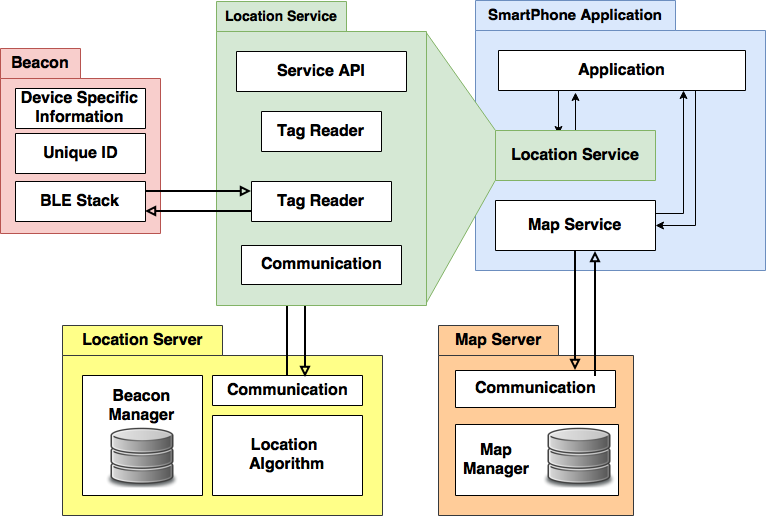
\includegraphics[width=1\linewidth]{figures/implementation.png} 
\caption[System's Architecture]{System's Architecture} 
\label{fig:implementation} 
\end{figure} 
 
 
\subsubsection{Bluetooth Low energy} 
\label{subsec:ble} 
 
For better understanding the beacon-smartphone communication, it is fundamental to comprehend how this technology works. All the presented information on BLE was obtained from its core manual \cite{BLECore}.  

The smartphone and the beacon are set up as two complementary classes. The beacon is defined as a peripheral, a role used to describe devices optimized to support a single connection. This role allows it to have a reduced complexity, since it's only required to function as a slave, an entity that is only capable of receiving connections. On the other hand, the smartphone is defined by the complementary role, central. A central device is capable of supporting multiple connections and is responsible for initiating all of them. 
 
\begin{figure} 
\centering 
\includegraphics[width=0.5\linewidth]{figures/profile.png} 
\caption[Gatt-based profile hierarchy]{Gatt-based profile hierarchy} 
\label{fig:profile} 
\end{figure} 
 
Another important aspect in understanding this technology is the BLE profiles. A profile, which can be seen on figure \ref{fig:profile} defines an hierarchy in which a device's available services are organized. By doing so, a system's profile ends up defining the applications behaviour and data formats, as well as the manner in which data is exchanged. The hierarchy is composed by two parts: Services and Characteristics. 
 
\begin{itemize} 
\item A profile is composed by one or more services. A service is a collection of data and associated behaviours to accomplish a particular function or feature of a device or portions of a device. It can be either primary, which provides primary functionalities of a device, or secondary, providing auxiliary functionalities of a device and being referenced from at least one primary service. A service is composed of characteristics and/or references to other services. 
 
 
\item A Characteristic is a value that is used in a service that has properties and configuration information that describe how the value should be accessed as well as information on how to display the value. A characteristic is defined by its declaration, its properties, its value and may also be defined by its descriptor, which describes the value or permit configuration of 
the server relative to the value. 
\end{itemize} 
 
\subsubsection{ BLE beacon} 
\label{subsec:beacon} 
 
 
The used beacons were Texas Instruments CC2650STK devices which can be visualised in figure ~\ref{fig:beacon}. Alongside the device, which comes with a pre-installed Bluetooth low energy program capable of giving information on each of its ten sensors through its predefined profiles, there is a texas smartphone application that can connect to a single device and read from its sensors. By using the texas Code Composer Studio (CSS), the predefined ble profile existent on the device could be altered. Upon further analysis of the profile, a characteristic was found for which the Universal Unique Identifier (UUID) of the service and the characteristic itself was found and as such this was the one that ended up being used to store the device's owner server's address. Since the device was already set to work as a peripheral and it now stored the information relevant to the system, there was no need to do further work. 
 
 
\begin{figure} 
\centering 
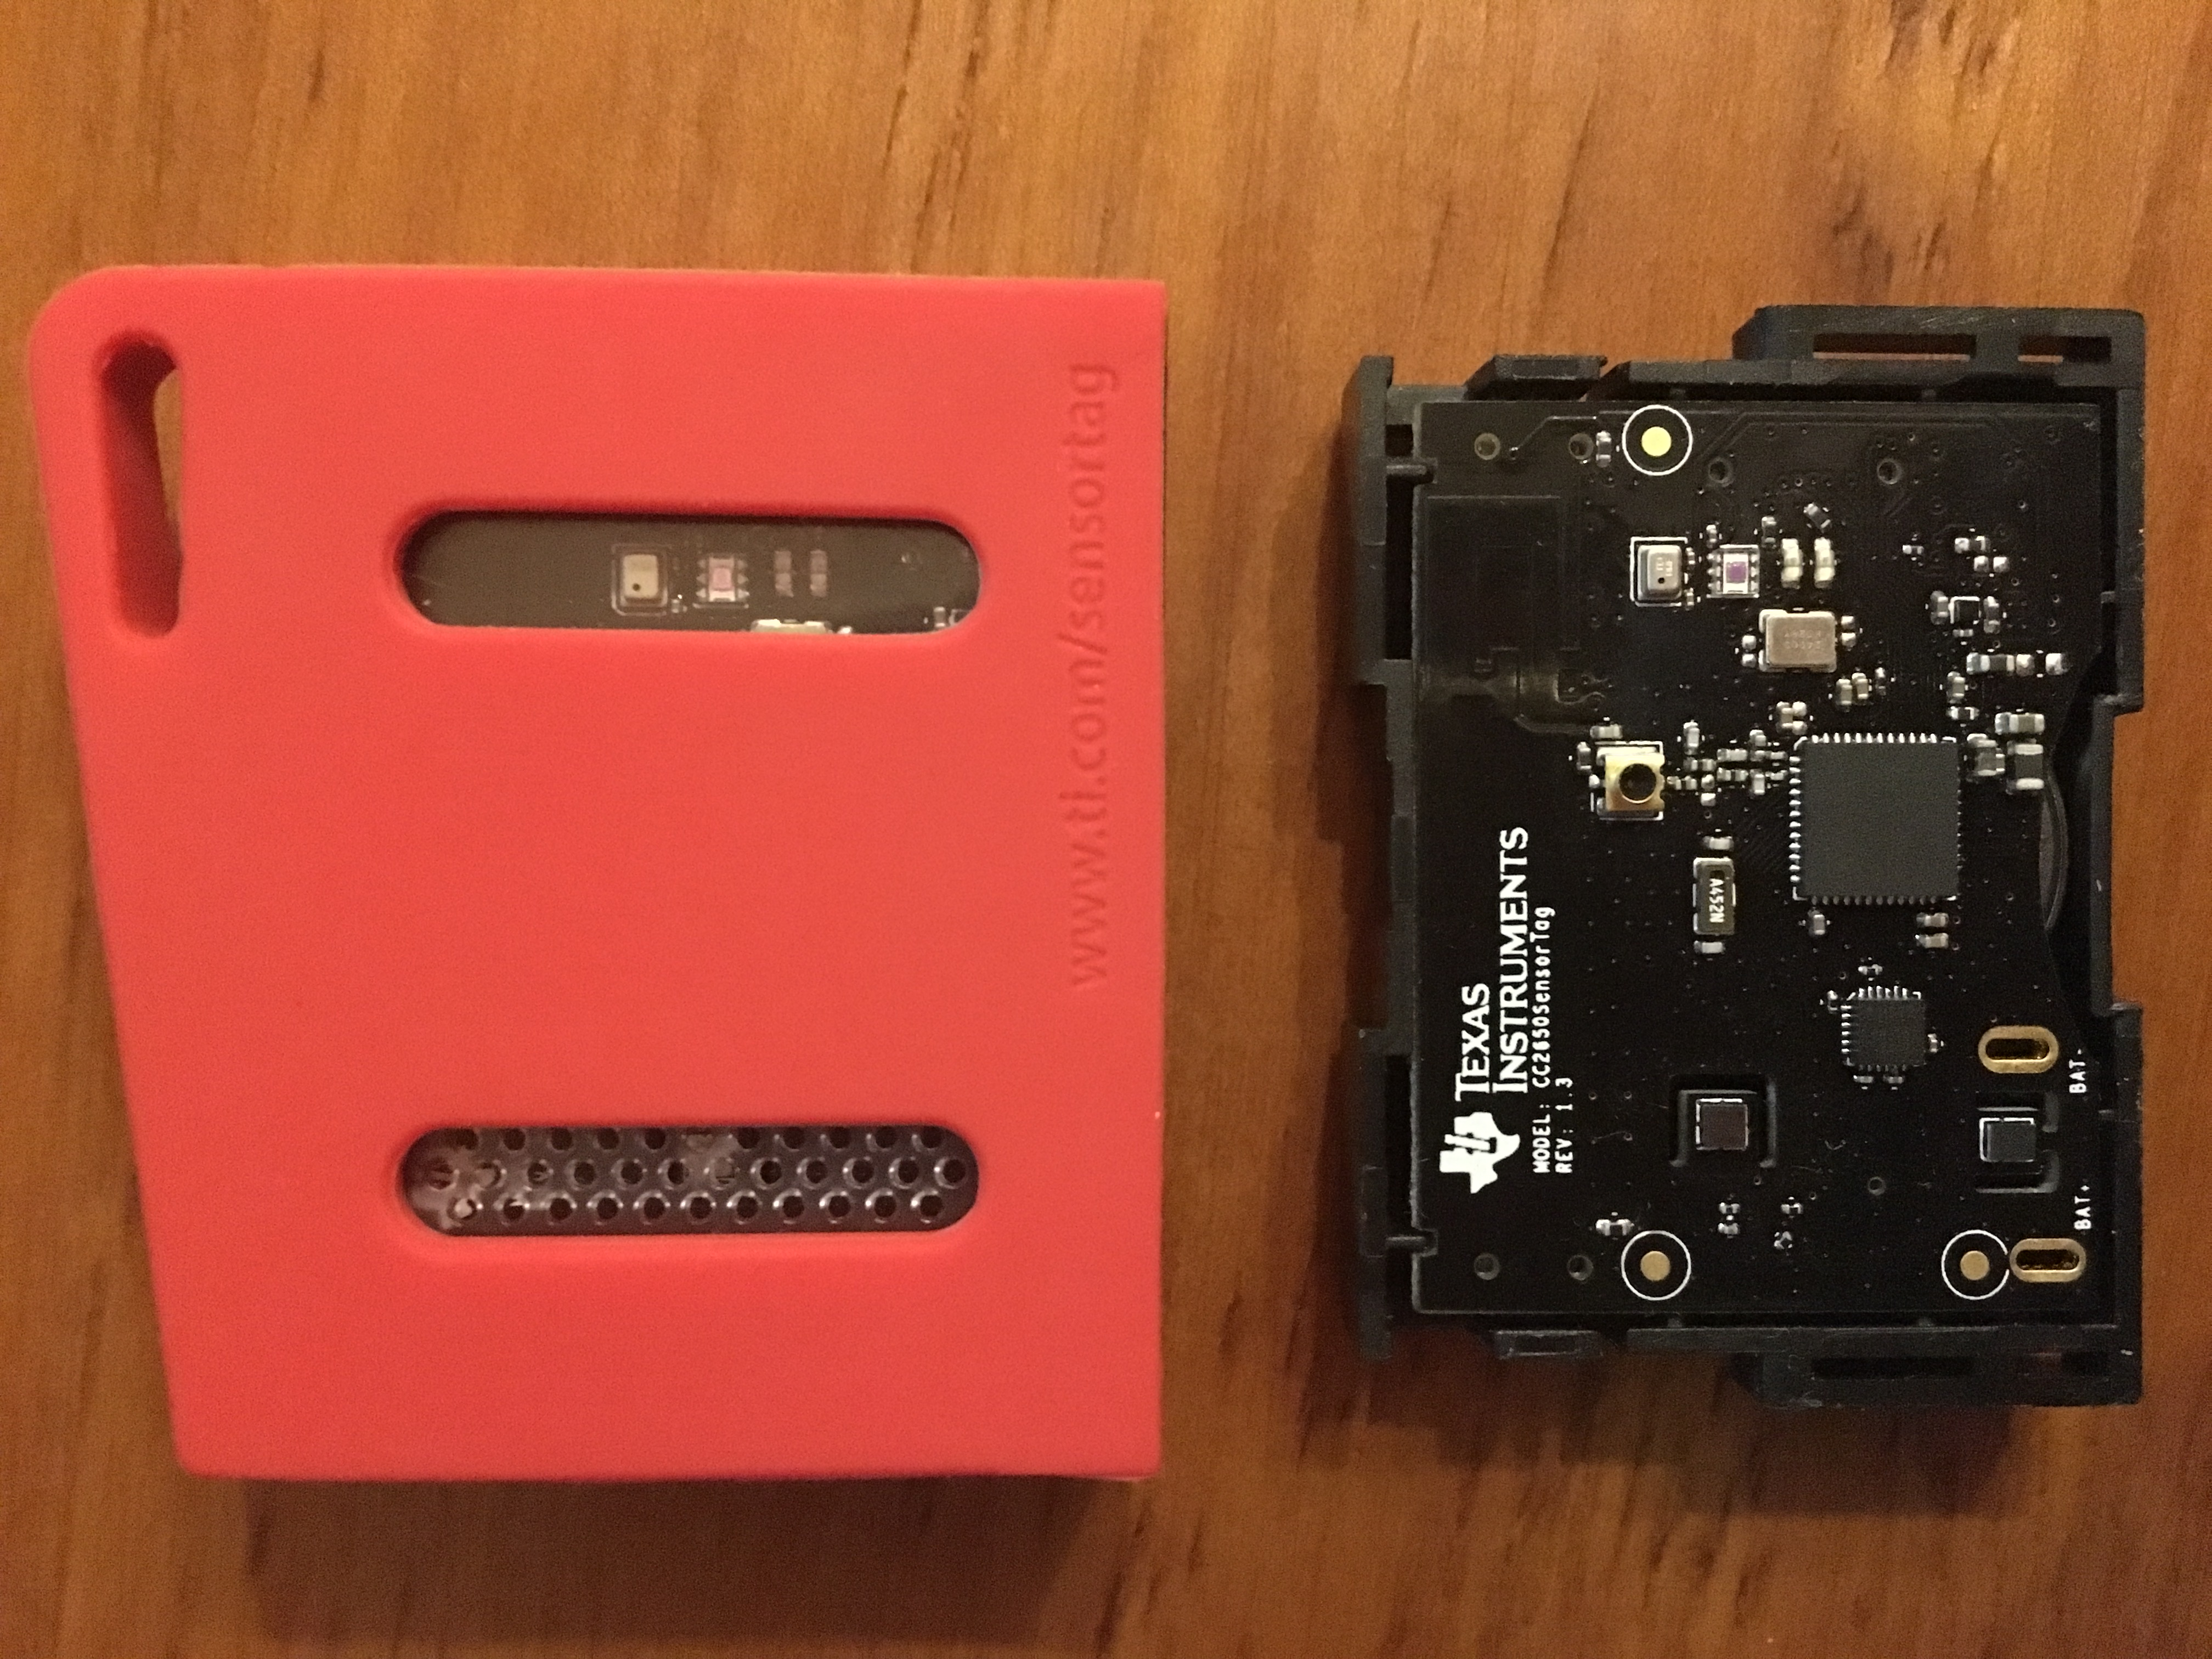
\includegraphics[width=0.5\linewidth]{figures/beacon.jpg} 
\caption[TI cc2650stk sensortag]{TI cc2650stk sensortag} 
\label{fig:beacon} 
\end{figure} 
 
 
\subsubsection{ Smartphone service} 
\label{subsec:service} 
 
 
The Smartphone application was developed for Android using the Android Studio IDE. The Application is divided in two primary functional blocks, the Mock location Provider and the Google Maps Integrated Display, as can be seen in figure ~\ref{fig:implementation}. 
 
 
The Mock Location Provider is implemented as if it was a Location provider, such as GPS. The application functions works as a listener to a Location provider, in this case it listens to the Mock Provider that was implemented. By implementing the whole process of obtaining a location inside a service (the mock provider) , a new level of abstraction is added to the application. As such, whenever the application is signaled to obtain the user's current location, a request is made to the associated location provider and the application only need to listen for the answer that eventually arrives. 
 
 
\begin{figure} 
\centering 
\includegraphics[width=0.5\linewidth]{figures/RequestLocation.png} 
\caption[Mock Location Provider Workflow]{Mock Location Provider Workflow} 
\label{fig:MockProvider} 
\end{figure} 
 
 
The Mock Location Provider incorporates the first three steps present in figure ~\ref{fig:MockProvider}, which will now be explored individually. The first step indicates the gathering of information of the surroundings of the user's device. When a request is made to the provider, a scan for nearby Bluetooth low energy devices is made. During this scanning period, each time a device is found, the advertisement is registered in a list, where a duplication prevention mechanism is implemented. Once the scanning is complete, the provider has available a list of all the ble devices within range.    
 
 
The second step involves taking the created list of devices, obtaining a server address and forwarding the same list to it. Once the first step is completed, the provider will analyse each entry at a time. For each device the provider will attempt to respond to the caught advertisement packet, resulting in a created connection.  Once the connection is created the provider asks for the available services of the paired device. Upon receiving an answer, the list of services is swoop while looking for the service with the wanted UUID. If the device doesn't have the UUID that the provider is looking for, it can assume that the paired ble is not a beacon of the system. When the provider identifies that the device has the system's UUID, it requests the device to hand over the service's existent characteristics. The provider will receive a list composed of the service's characteristics and it will search in it for the system's characteristics UUID, the one which contains the device's server's address. This search has the objective of confirming that the service present in this device is indeed the one that was implemented for the system and not a service that happened to have the same UUID. For any service outside those that are documented in the Bluetooth Special Interest Group (SIG), who have a specific UUID attached to them, the UUID is generated randomly and as such there is a small chance of collision. Once the wanted characteristic is found, the provider requests the device to read its value and stores the received value in a list. This list will contain the servers of the devices that were found, and for each address there will be a list corresponding to each device, as well as their corresponding RSSI values. In order to quicken the previously described process, the provider keeps in cache the most recent contacted devices. Before attempting a connection, the provider confirms that the device isn't found in cache and when finishing a process, the associated device is inserted into the cache. 
 
 
When every device has been contacted, a voting system is actioned which will decide from the list of servers which one it will send the collected information to. The voting system uses an exponential function in order to attribute a weight to each server.  
 
 
The voting system was implemented with the objective providing a thin security layer by allowing multiple devices of the same server to overcome a single attacker's device which happened to be close to the user. After obtaining each server's values, the one with the highest value is chosen and sent the list with all the devices.  
 
 
The Third step involves a simple client/server tcp interaction. The application starts off by creating the message that it will later on send to the server. This message includes all pairs of device mac address and its associated rssi value captured by the application on the first step. Consequently, the application attempts to create a connection with the server at the chosen address at the end of step two. With the connection established, the message is forwarded to the server and the application is put onto blocked state where it awaits for an answer. Upon arrival, the answer received is checked for valid location, its information process and the connection terminated. The information contained inside the received message, which was described in section ~\ref{subsec:server}, is then processed into the adequate class capable of storing a geographic location and the same is broadcasted from the mock location provider to its listener.  
 
 
 
 
The Google Maps Integrated display is implemented using the Google Maps Android API. By using Google Maps it was possible to alleviate the weight on the application since there was no to implement a maps server.  By making this development choice, the system as a whole became closer to the desired generic approach while making possible for seamless transition between indoor/outdoor maps. The only imposed restriction is related to the addiction of new indoor maps onto the google maps, which is possible and well documented but dependent on a third party. 
 
 
The Fourth step is called when the application receives a proper location from the request made onto the location provider. With the device's location known, a marker is placed on the map with the obtain coordinates (longitude, latitude), the camera is moved in order to be centered on the position, while fully displaying the indoor level map. The menu visible on figure \ref{fig:AppMenu} is also updated with the information that is bundled with the received location. In order to show the correct level on a multi level building, the "floor" information present in the menu is used. The API allows for obtaining a list of existent levels on which the maps' camera is focused. As such it's possible to find out to which level the provided location belongs, as well as displaying it to the user. 
 
 
 
 
\subsubsection{ Server} 
\label{subsec:server} 
 
 
The web server was implement in Python 3 programming language. The program implements a simple tcp server capable of receiving multiple request at the same time. Each request starts with information sent from an application which include a pair of MAC address and associated RSSI value for each ble device that the same application found. Afterwards the list of pairs is filtered in order to remove any existent devices that are not present in the server's database of devices. 
 
 
Each server has a database that includes only ble devices. An entry (description of a device) in this database is composed by the device's mac address, its longitude and latitude and its building, floor and room name. In addition to the database, a server can store additional location info such as the server's street, number, zip-code, city and country, allowing this information to be transmitted to the client, thus offer an additional level of location description to the user. The whole location specific information can be visualised in figure ~\ref{fig:AppMenu}. 
 
 
Upon having filtered the initial list of pairs, the Cell of Origin (CoO) technique is applied by verifying which of the devices produced a stronger signal on the receptor. Upon obtaining the closest device, an answer is sent to the application containing all of the information associated to the server and the selected device. 
 
 
\subsection{Evaluation} 
\label{sec:eval} 
 
The pop-up menu was implemented to demonstrate the capacity of providing additional information associated with each location, be it geo-location taxonomy as it is currently implemented or possibly a description of the located room, an hyperlink of some sort or any other type of data that someone implemented this system would like to provide to its users.   
 
 
The final state of the implemented system can be visualised in figure ~\ref{fig:AppFocus} and figure ~\ref{fig:AppMenu}. The first displays the case of obtaining a location, where the marker has been placed and the camera zoomed. 
 
 
\begin{figure} 
\centering 
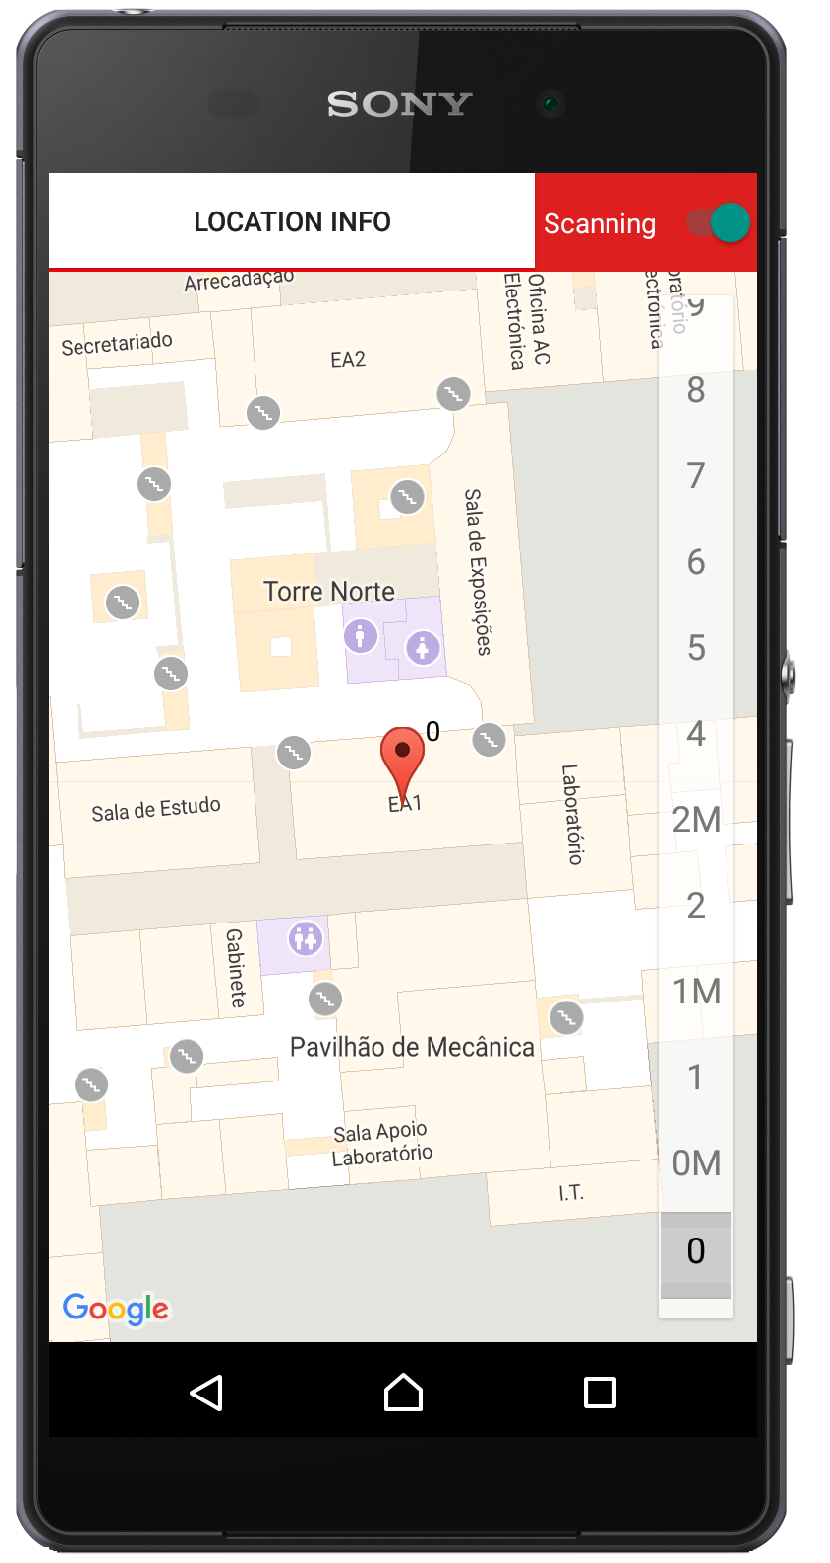
\includegraphics[width=0.5\linewidth]{figures/app_focused.png} 
\caption[Application screen showing a focused location on a room]{Application screen showing a focused location on a room} 
\label{fig:AppFocus} 
\end{figure} 
 
 
\begin{figure} 
\centering 
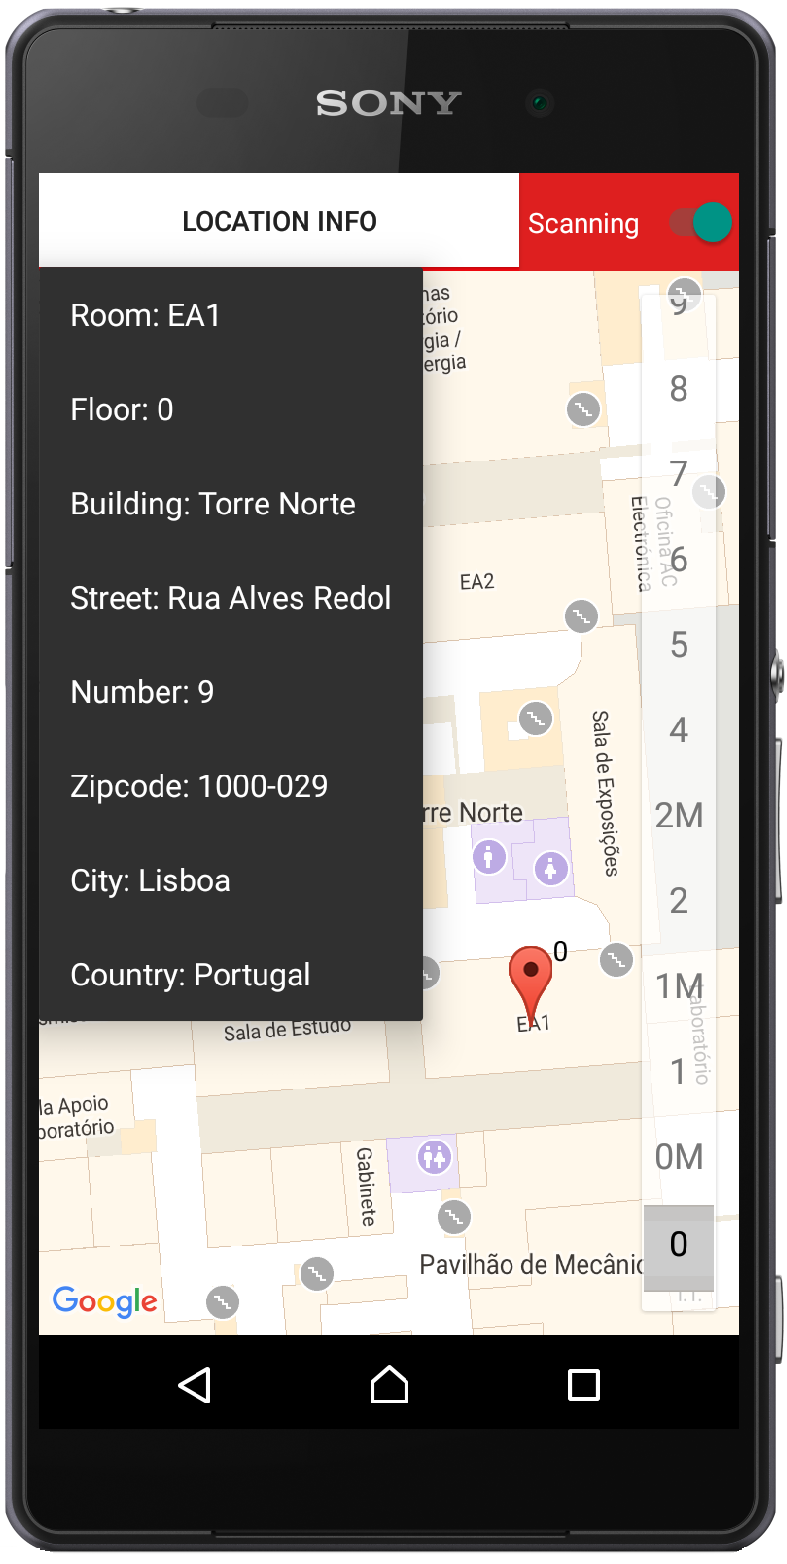
\includegraphics[width=0.5\linewidth]{figures/app_focused_menu.png} 
\caption[Application screen showing additional information of location]{Application screen showing additional information of location} 
\label{fig:AppMenu} 
\end{figure} 
 
 
 
 
In order to analyse the energetic costs of the BLE system implementation a series of tests were planned and executed. The tests were conducted with the intention of discovering the costs of the smartphone on standby, the overall cost associated with the system as well as the ones associated to the communication process.  
 
 
The used smartphone was a Sony Xperia E5, whose battery is rated at 2300 mAh. The battery values data collection was made through the android API, which allows one to know the battery percentage of the smartphone. 
 
 
The tests were all conducted under the same base conditions, the battery was completely charged, without a SIM card and with the screen at maximum brightness. They were also conducted over the period of an hour. 
 
 
The first batch of tests, presented in figure \ref{fig:syson}, display how the smartphone behaves without the system. The first test case shows the energetic costs for the smartphone on standby, i.e. with all sensors inactive, test \#2 occurs with the Wi-Fi active and without service, while test \#3 was performed with service available. The last test case \#4 is useful since it provides the consumption associated to having all the sensors active (Wi-Fi and Bluetooth). This value will allow for a better analysis of the system's performance. 
 
 
\begin{figure} 
\centering 
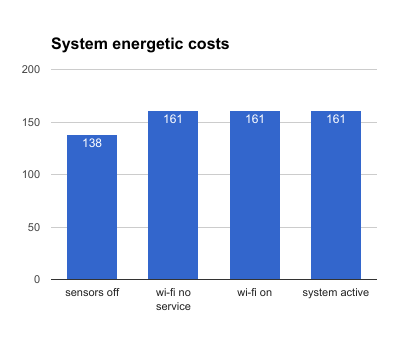
\includegraphics[width=1\linewidth]{figures/system-on.png} 
\caption[Test case \#1-4: System's energetic costs]{Test case \#1-4: System's energetic costs} 
\label{fig:syson} 
\end{figure} 
 
 
The second batch of tests, presented in figure \ref{fig:syswork}, allowed for the system's operational costs to be analysed. As seen in the figure, the parameter that is being tuned is the operation's cycle period, 5,15,30 and 60 seconds, which is tested with one and two devices.  
Through these tests it is possible to visualise the impact of the number of operations on the battery, which is proportional to the number of devices. Passing from one to two devices leads to an increase in the order of the 1\% of the total battery. This is caused by the increased cost of the BLE communication, since the systems is required to query one extra device each cycle. 
 
 
\begin{figure} 
\centering 
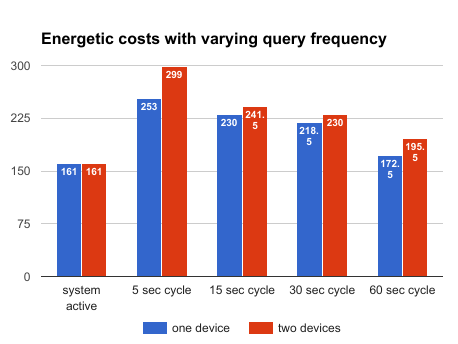
\includegraphics[width=1\linewidth]{figures/system-working.png} 
\caption[Test case \#5-12: System Working - energetic costs]{Test case \#5-12: System Working - energetic costs} 
\label{fig:syswork} 
\end{figure} 
 
 
In order to better understand the costs associated with the BLE communication component, it is necessary to also understand the costs associated to the network component, i.e. communication with both servers. Figure \ref{fig:commcosts} allows one to do that, since it shows side-by-side the cost of the whole operation cycle and the costs of the operational cycle without the network communication, i.e. the cycle is concluded after concluding the BLE communication. The other factor that is tuned is the number of devices which turnout out to be relatively irrelevant since the message's complexity grows slowly with the increase in the number of devices.  
 
 
\begin{figure} 
\centering 
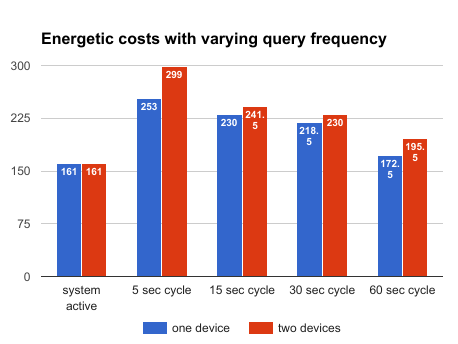
\includegraphics[width=1\linewidth]{figures/system-working.png} 
\caption[Network Communication's Energetic cost]{Network Communication's Energetic cost} 
\label{fig:commcosts} 
\end{figure} 
 
 
Although the operational costs can seem rather high, the test context isn't implement with any of the possible optimisation techniques. When analysing the BLE communication costs, one has to be aware that in each cycle the beacons were contacted, meaning that if the associated address would be kept, only on query would be necessary. A small cache-like optimisation would heavily reduce the system's weight, making it so that only new devices would be required to be queried for their owner's server address. Regarding the network communication costs, they can be reduced by making use of other sensors to discover when the user is moving, so that only then the positions is searched for, as well as making optimisations regarding the maps component, such as not requesting the same locations multiple times.  
 
 
%% Qualitativamente 
 
 
Although a complete implementation of the proposed architecture was achieved for BLE, one must indicate the required changes that would be necessary to make when change one or several parts of the system. The parts that can be changed are the three possibilities previously studied from figure \ref{fig:choices}. In case the technology is to be change, we will use QR code as an example, the affected areas are the beacons, the smartphone service and the location server. By changing to QR codes, the technology changes instantly as there is no more requirement for BLE beacons, but instead there will be QR codes placed in fixed places. Each QR code would be required contain information about its associated server. The service would change the mechanism used to collect data, instead of listening for BLE beacons through its Bluetooth antenna, it will open up the camera, so that the user can capture the QR code. The location server would have to be prepared to receive the QR data and obtaine the location relative to that QR code. 
 
 
If the system was to be changed on the location algorithm component, this would only require changes on the location server. The algorithm component has only two connections points with the system, the data that it receives and the location it outputs. As such, for as long as the new algorithm makes use of the same data and in the end, once it has concluded, it outputs one location of the same format, no other issue should surface. 
 
 
A modification on the location description would have an impact on both the location and map server. With such a request, the map server is required to change completely the stored maps in order to support the new description method, while the changes on the location server are on the database, since the location of the beacons should change, and on the way the location algorithm processes these same locations.   
 
 
\section{Conclusions} 
\label{sec:conclusions} 
 
 
In this paper, one has presented GEFILOC, a generic framework architecture for indoor location systems centered around smartphones. This architecture intended to present a common ground for the many existing indoor location systems, where the central piece of communication would be the smartphone. By making it the central component and using its sensors, one is capable of externalising the different components of a generic indoor system. This allows for higher scalability, as well as interoperability between different systems. 
 
 
An implementation of the architecture was achieved through the usage of the Bluetooth low energy technology and the Android operating system. The implemented system was successful, having achieved communication between beacons and smartphone, having implemented a location server capable of host the beacon's data and any location algorithm, and having achieved incorporation of the google maps as its maps provider. 
 
 
The energetic costs associated to the implemented system were promising although for a complete understanding of its cost in a fully-developed system, a more optimised version would be required. Despite this factor, the most relevant cost was the one associated to the network, since it came as a tradeoff for the scalability, which didn't achieve concerning values. 
 
 
These results indicate that it could be possible to use this architecture in multiple indoor location systems and eventually integrating them into the same smartphone application service. This situation would allow users to navigate through buildings, while interacting with whichever system is associated to his vicinity. 
 
 
\bibliographystyle{IEEEtran} 
\bibliography{paper} 
 
 
\end{document} 